\chapter{Methodology}
\label{chap:2}
\ChapterPageStuff{2}

\section{Preamble} The literature in \Cref{chap:1} is used for the method to create a logging mechanism that can capture user-based activity logs to improve software maintenance by analysing the obtained logs. The web-based application system on this logging mechanism will be implemented on is an energy management system for the mining industry.\par In \Cref{Ch2:LoggingMechanism} the methodology to create a logging mechanism to capture user-generated events is discussed for web-based applications. The different functional requirements and interfaces are discussed in this section \cite{Anish2015}.\par In \Cref{ch2:system_utilisation_analysis} the methodology is discussed to analyse these obtained logs to improve software maintenance.

\section{Logging mechanism}\label{Ch2:LoggingMechanism} The logging mechanism will need to meet the requirements discussed in \Cref{sec:EventLogging} to capture the required logs to apply system utilisation analysis on it. \Cref{fig:ch2:systemDesign} is the design for the logging mechanism to capture the user's activities. In this figure, the logging mechanism is split up into two functional requirements parts (F/R) which consist of the client and server functional requirements.\par Each functional requirement has an interface requirement that transfers the data from one interface to another interface. These interfaces are labeled as I/F in \Cref{fig:ch2:systemDesign}. The \Cref{fig:ch2:systemDesign} is the client interface (F/R 1) and the server interface (F/R 2) that forms the entire logging mechanism to capture the user-based activity logs.

\begin{figure}[!htb] % An h :here, t: top, b: bottom.
	\centering % cent the figure
	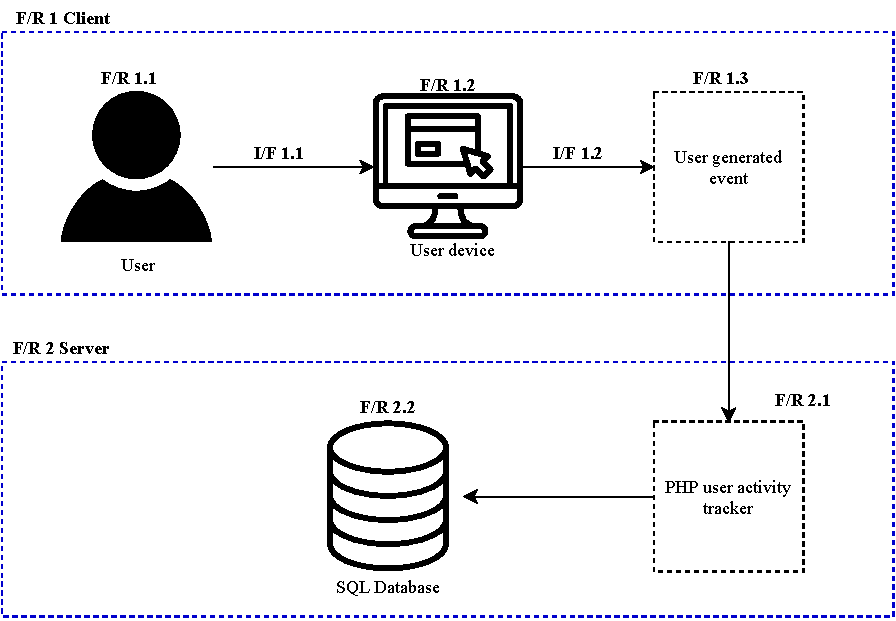
\includegraphics[width=0.9\textwidth]{Chapter2/SystemA_Architecture_Diagram/SystemA_Architecture_Diagram.pdf}
	\caption[Logging mechanism architecture design]
	{\textit{Logging mechanism architecture design}}\label{fig:ch2:systemDesign}
\end{figure}

\clearpage

\subsection{Clients functional requirements}

The client's functional requirements (F/R 1) are where the user-based activity is triggered. In \Cref{fig:ch2:systemDesign} the client interface consists of three main functional requirements. These interfaces in \Cref{tbl:ch2:clientFunctionalRequirements} parses the input from the user to create a basic user event log. 

\begin{table}[!htb]
	\centering
	\small
	\caption[Client functional requirements]
	{\textit{Client functional requirements (F/R 1)}}
	\label{tbl:ch2:clientFunctionalRequirements}
	\begin{tabularx}{\textwidth}{|l|l|X|}
		\hline \textbf{Requirement ID} & \textbf{Name} & \textbf{Description} \\
		\hline F/R 1.1 & User & The user serves as the primary initiator of the activity events.\\
		\hline F/R 1.2 & User's device & The device that the user uses to access the website from where the activity events are generated.\\
		\hline F/R 1.3 & User-generated events & These are any activity events that the user started that need to communicate back to the server.\\
		\hline
	\end{tabularx}
\end{table}

\subsection{Requirements for a user-based activity log}
The user is the initiator of the logging mechanism. Each action or event they trigger by interacting with the user interface on their device (F/R 1.2) can be a potential user-generated event. In
\Cref{tbl:ch2_requirementsForUserActivtyEvent} is the sub-requirements for the user (F/R 1.1) which the event log should fulfill to be classified as an user-based activity log.

\begin{table}[!htb]
	\centering
	\small
	\caption[Requirements for an event to be a user-based activity]
	{\textit{Requirements for an event to be a user-based activity}}
	\label{tbl:ch2_requirementsForUserActivtyEvent}
	\begin{tabularx}{\textwidth}{|l|X|}
		\hline \textbf{Requirement ID} & \textbf{Description}\\
		\hline F/R 1.1.1 & The event has to be triggered by the user interacting with the user interface using their device. \\
		\hline F/R 1.1.2 & The event must consists of different cases ($ca~ \epsilon~CA$ the cases consists of events) which are noteworthy to make the event log identifiable \cite{Slaninova2014}. \\
		\hline F/R 1.1.3 & For certain types of event logs for F/R 1.1.2, the user-generated event should have an origin from which the event took place. \\
		\hline F/R 1.1.4 & The event log should consist of attributes that expand the identity of the user-based activity. \\
		\hline F/R 1.1.5 & The event must have the user as the initiator or input for the user-based activity. This will exclude all events triggered by the system as the user did not directly start the event.\\ 
		\hline
	\end{tabularx}
\end{table}

Every interaction the user has with the user interface of the device to the software system can be seen as an event triggered by the user. Most of these events won't have a meaningful impact as they won't fulfill F/R 1.1.2 and F/R 1.1.4 in \Cref{tbl:ch2_requirementsForUserActivtyEvent}.\par For the user activity event to meet the requirement of 1.1.2 it has to have defined cases that describe the activity type of each event. These activity types form the basic criteria for which event can be parsed which significantly reduces the number of logs that will be obtained. This will ensure that the event logging process will produce quality user-based logs as discussed in \Cref{sec:ch1:loggingQuality}:

\begin{itemize}
	\item A basic structural complexity to simplify log parsing,
	\item Increase accuracy by only obtaining the logs that are part of the different defined cases,
	\item Keep the logging consistent by not deviating from the defined cases, and
	\item Ensure that the event log's other attributes are complete and available
\end{itemize}

\subsection{Web application architecture}\label{sec:ch2:webApplicationArchitecture}
To determine the user activity types for a Web application, the Web application's architecture will be a factor in the logging mechanism. Web applications consist mostly of HTML, JavaScript and CSS programming languages. The Model-View-Controller (MVC) architecture is mostly used for web-based applications using that programming language \cite{Jailia2016}. The MVC architecture in \Cref{fig:ch2_flowMVC_Architecture} consists of 3 basic parts which are the \cite{Jailia2016}:

\begin{itemize}
	\item \textit{Model:} Is the representation of the records in the database which also interacts with the database through a database access layer or service manipulating the data by using:
	\begin{itemize}
		\item \textit{create} operation that adds new data,
		\item \textit{update} operation that modifies the existing data,
		\item \textit{delete} operation that removes data.
	\end{itemize}
	\item \textit{Controller:} Is operates both the \textit{View} and \textit{Model} and serves as the connection between the user and the system by controlling the data flow of the \textit{Model} and
	\textit{View}.
	\item \textit{View:} This shows the results of the data contained in the \textit{Model} and enables the user to manipulate the data. The user will only interact with this part of the Web application.
\end{itemize}

\begin{figure}[!htb] % An h :here, t: top, b: bottom.
	\centering % cent the figure
	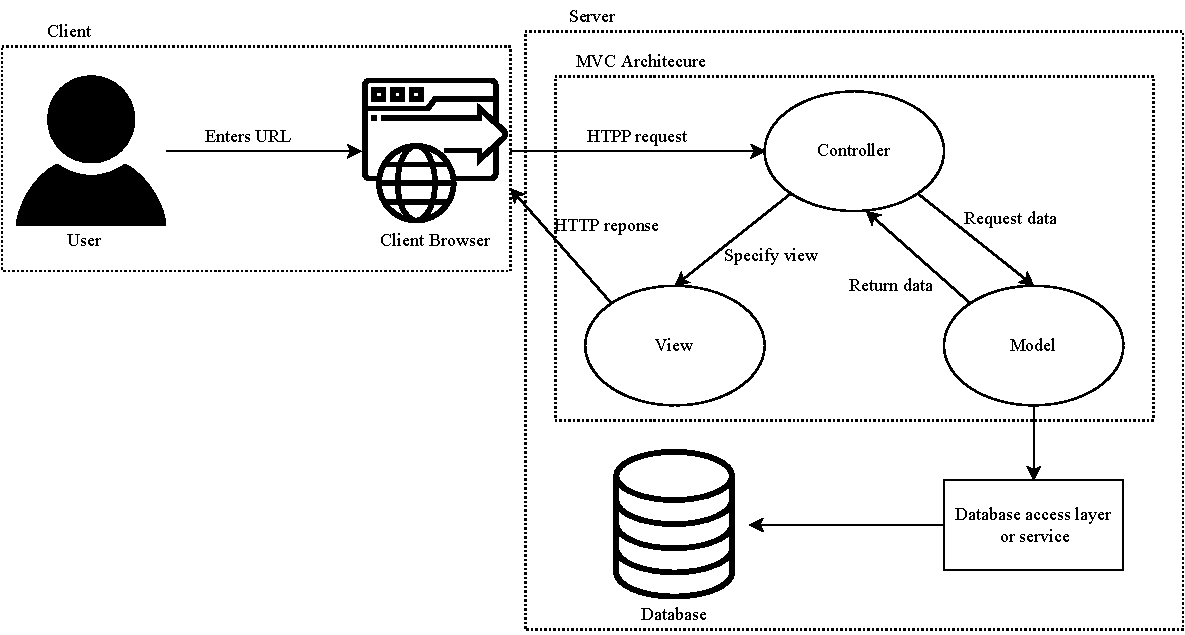
\includegraphics[width=0.9\textwidth]{Chapter2/Flow_MVC_Architecture/Flow_MVC_Architecture.pdf}
	\caption[MVC architecture for most web-based applications]
	{\textit{MVC architecture for most web-based applications \cite{Gu2010}}}\label{fig:ch2_flowMVC_Architecture}
\end{figure}

In \Cref{fig:ch2_flowMVC_Architecture} is the MVC architecture equivalent representation of \Cref{fig:ch2:systemDesign} where the data flow is shown of the MVC architecture. The user interacts with the Web application through their browser which will send a \textit{HTTP requests}\footnote{A \textbf{HTTP request} is made by a client, to a named host, which is located on a server. The request aims to access a resource on the server. \cite{IBM2021}.} to the \textit{Controller} and receive a \textit{HTTP response}\footnote{An \textbf{HTTP response} is made by a server to a client. The response aims to provide the client with the resource it requested, inform the client that the action it requested has been carried out; or else inform the client that an error occurred in processing its request. \cite{IBM2021a}.} from the \textit{View}.The \textit{Controller} will request and return the data to the \textit{Model} which interacts with the database access layer or service to do the \textit{create}, \textit{update} and \textit{delete} operations.\par To classify any interaction between the user (F/R 1) and server (F/R 2) to fulfill the functional requirements of \Cref{tbl:ch2_requirementsForUserActivtyEvent} only the \textit{HTTP request} are used for the logging points in \Cref{sec:ch2:loggingPoints} as it:

\begin{itemize}
	\item Meet the F/R 1.1.1 and F/R 1.1.5 as the user will interact with the \textit{View} to modify the data which needs to send back an \textit{HTTP request} to process the data on the \textit{Controller}.
	\item User activity types can be catered for certain scenarios when the request is being sent.
	\item Any additional metadata can be sent with the \textit{request header}\footnote{A \textbf{request header} is an HTTP header that can be used in an HTTP request to provide information about the request context so that the server can tailor the response. For example, the Accept-$\ast$ headers indicate the allowed and preferred formats of the response. \cite{Mozilla2022}.} of the \textit{HTTP request}. This will reduce the overhead added by the logging mechanism by not sending additional \textit{HTTP request} each time back to the server when a user-based activity has been identified.
\end{itemize}

\subsection{User activity types}\label{sec:ch2:userActivityTypes}
The user-activity logs will be split into three main event types as in \Cref{tbl:ch2:userActivityTypes}. The general user activity event type (F/R 1.2.3) will the be most common user activity event and be split up into different user activity events. This is determined by the need of what utilisation stage requires to analyse specific user activity events. 

\begin{table}[!htb]
	\centering
	\small
	\caption[User activity types]
	{\textit{User activity types}}
	\label{tbl:ch2:userActivityTypes}
	\begin{tabularx}{\textwidth}{|l|l|X|}
		\hline \textbf{Requirement ID} & \textbf{Activity Type} & \textbf{Description} \\
		\hline F/R 1.2.1 & Web page accessed & The user may navigate through different web pages in a session.\\
		\hline F/R 1.2.2 & Session changes & This is any user activities that directly involve an extension session before their session times out after a period of inactivity. This also tracks when
		the session starts as any login attempt is a user-based activity.\\
		\hline F/R 1.2.3 & General activity & Any events excluding the first two user activity types that the user initiates when they interact with the web page. Most of the user activity logs will
		have this event type.\\ 
		\hline
	\end{tabularx}
\end{table}

\subsection{Logging points and log attributes}\label{sec:ch2:loggingPoints}
In \Cref{sec:ch1:loggignPoints} the logging points should be strategically placed in the software system to capture the log attributes for the user-based activity log. To meet the requirements of \Cref{tbl:ch2_requirementsForUserActivtyEvent} for a user-based activity the logging points should adhere to the logging points functional requirements of \Cref{tbl:ch2_loggingPointRequirement}.

\begin{table}[!htb]
	\centering
	\small
	\caption[Logging points requirements]
	{\textit{Logging points requirements}}
	\label{tbl:ch2_loggingPointRequirement}
	\begin{tabularx}{\textwidth}{|l|X|}
		\hline \textbf{Requirement ID} & \textbf{Description} \\
		\hline F/R 1.3.1 & The logging point should be placed where the user's interaction with the software system will send a \textit{request} back to the server.\\
		\hline F/R 1.3.2 & Each logging point should consistently capture the user-based activity as the activity is happening. \\
		\hline F/R 1.3.3 & Logging points should be globally complete to capture the user-based activities in the giving software system without too much modification between each point in the same
		software system. \\
		\hline F/R 1.3.4 & The logging points should not interfere with the rest of the system's operations, this would be slowing down the system by causing too much overhead in each \textit{request}
		that is being sent. \\
		\hline
	\end{tabularx}
\end{table}

%To meet the F/R 1.3.1 the logging point should be placed where the logging point can determine the event that has been triggered by the user (F/R 1.1.1). 

The defined logging attributes in \Cref{tbl:ch2:keyLoggingAttributes} are the base attributes that form part of the main structure of the user-based event log. For web-based applications on the
client side, only some of these attributes can be obtained as the rest of the attributes can be resolved on the server side. The metadata (F/R 1.4.6) can consist of the request parameters that are
obtainable at the server side but any additional captured data can be added and sent to the server. A default activity type (F/R 1.4.3) can be set at the logging point. 

\begin{table}[!htb]
	\centering
	\small
	\caption[Key logging attributes]
	{\textit{Key logging attributes}}
	\label{tbl:ch2:keyLoggingAttributes}
	\begin{tabularx}{\textwidth}{|l|l|X|}
		\hline \textbf{Requirement ID} & \textbf{Logging point} & \textbf{Description} \\
		\hline F/R 1.4.1 & Identification number & The activity identification is an incremental number of the user-based event that is logged.\\
		\hline F/R 1.4.2 & Timestamp & This is the time the user initiated the user-based activity event.\\
		\hline F/R 1.4.3 & Activity type & Each event can be classified into user-based types. This is the user-based activity types in \Cref{tbl:ch2:userActivityTypes}.\\
		\hline F/R 1.4.4 & User identification & Each user has a unique identification number that links the event to them. \\
		\hline F/R 1.4.5 & Request origin & In web applications, there are always requests sent back to the server and will call the primary function to handle the request. The file in which the
		the function is the request origin. \\
		\hline F/R 1.4.6 & Metadata & The metadata of the event contains request parameters or other relevant request data of the event. This metadata adds more information about the user's activity.
		In \Cref{fig:Ch2_Metadata_Json_Example} is an example representation of the metadata. \\
		\hline F/R 1.4.7 & Miscellaneous attributes & These are any non-metadata attributes that can be consistently captured to be used in the utilisation analysis.\\ \hline
	\end{tabularx}
\end{table}

\clearpage
Each of these log attributes combined creates the base log from which key logging points can be created in the software system to capture the user-based activity logs. The 

\begin{figure}[!htb]
	\centering
	\begin{lstlisting}[style=json] 
		{ "RequestOrigin" : "/Area4/Controller4",
		  "RequestElementID" : "Button4",
		  "RequestParameters": {
		  "Parameter1": 4,
		  "Parameter2": "Hello World!",
			"Parameter3": true
			"Parameter4": 40.404
		  }		
		}
	\end{lstlisting}
	\caption[Metadata JSON]
	{\textit{Metadata JSON}}\label{fig:Ch2_Metadata_Json_Example}
\end{figure}

\clearpage

\subsection{Client functional requirements interaction}
\par In \Cref{fig:ch2_user_based_actvity_classification} is the complete process of the user interacting with the UI to trigger a user-based activity event to be logged later for the client's functional requirements. It starts with the user interacting with the user interface. The potential user activity needs to meet the first requirement (F/R 1.1.1) of \Cref{tbl:ch2_requirementsForUserActivtyEvent} or else it should be not be logged. The default activity type is set to general activity (F/R 1.2.3) until it is further processed later in the logging mechanism.\par If the activity has any additional metadata such as the request parameters, it will also be logged. The other metadata can also be captured in this stage from the client side like the element that the user clicked on to start the event.

\begin{figure}[!htb] % An h :here, t: top, b: bottom.
	\centering % cent the figure
	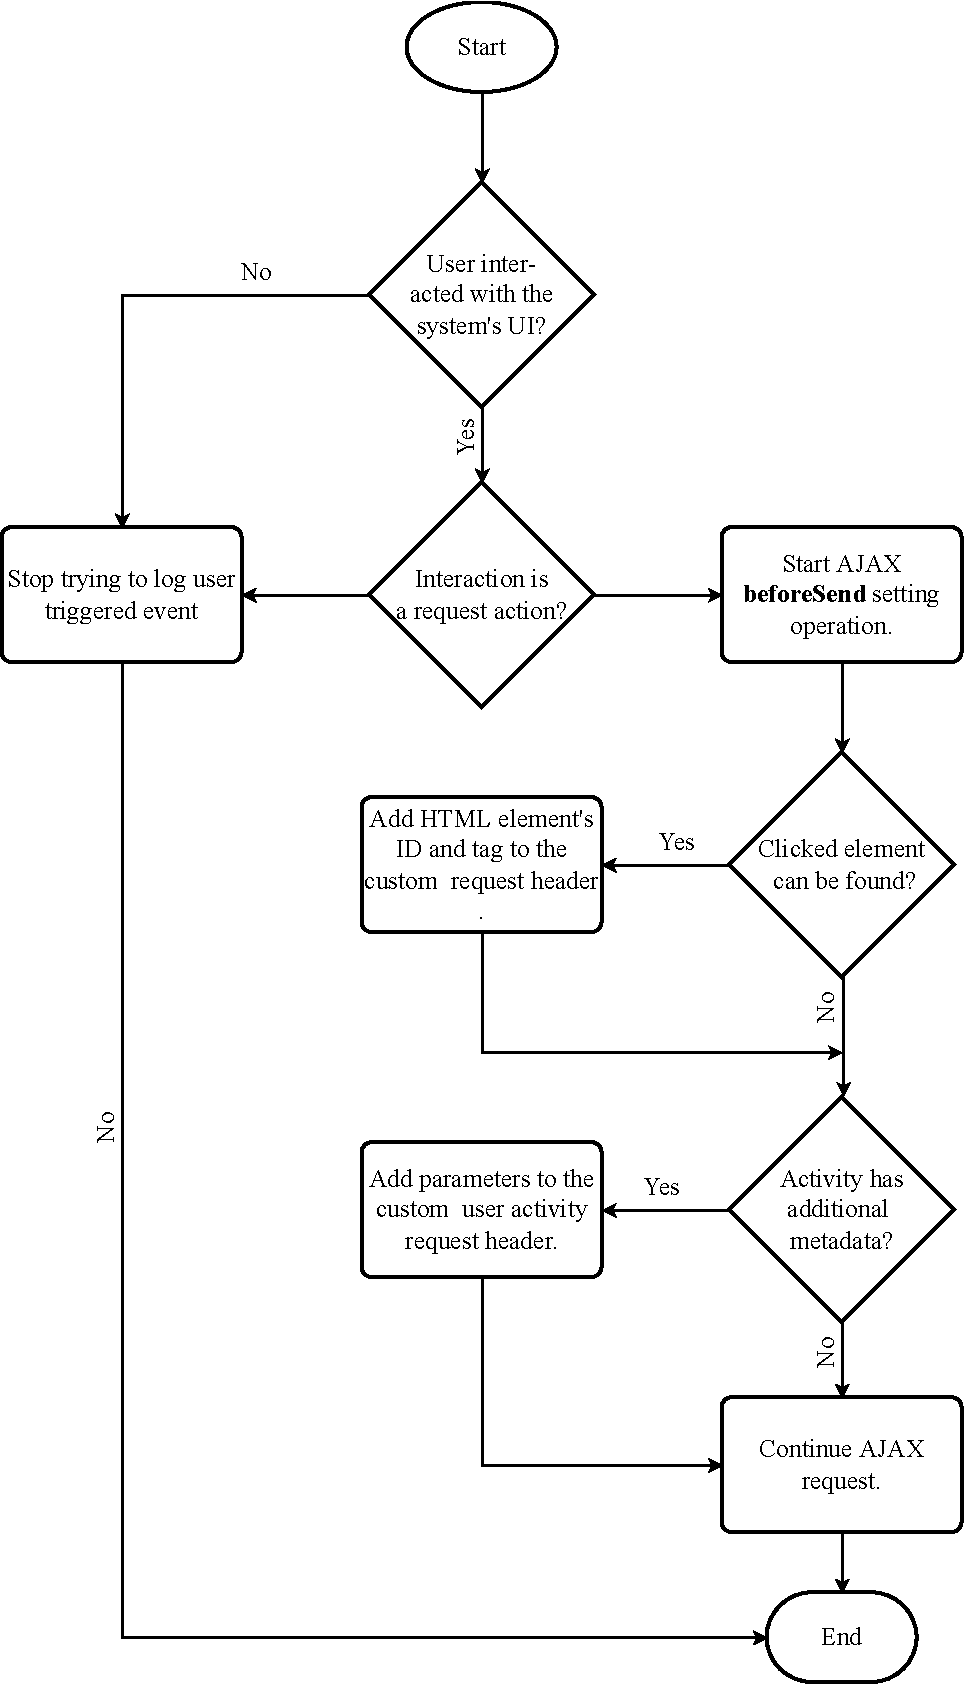
\includegraphics[width=0.6\textwidth]{Chapter2/client_functional_requirement_flow_diagram/client_functional_requirement_flow_diagram.pdf}
	\caption[User-based activity log classification flow diagram]
	{\textit{User-based activity log classification flow diagram}}\label{fig:ch2_user_based_actvity_classification}
\end{figure}

\clearpage

\subsection{Server's functional requirements}
The server functional requirements in \Cref{tbl:Ch2_Server_Functional_Requirements} for \Cref{fig:ch2:systemDesign} is the rest of the logging mechanism. At this stage, the obtained user-generated event of \Cref{fig:ch2_user_based_actvity_classification} will be attempted to be completed into a user-based activity log and stored in a database.

\begin{table}[!htb]
	\centering
	\small
	\caption[Server functional requirements]
	{\textit{Server functional requirements (F/R 2)}}
	\label{tbl:Ch2_Server_Functional_Requirements}
	\begin{tabularx}{\textwidth}{|l|l|X|}
		\hline \textbf{Requirement ID} & \textbf{Name} & \textbf{Description} \\
		\hline F/R 2.1 & User activity logger & The key logging points are used to capture and create the user-based event log that will be stored in a database.\\
		\hline F/R 2.2 & Database & The event log is stored in a database until it is needed for further analysis.\\
		\hline
	\end{tabularx}
\end{table}

The interfaces in \Cref{tbl:ch2:serverInterfaceRequirements} for the client functional requirement (F/R 2) is to obtain the base log from the client functional requirement (F/R 1) and finally store the completed log into a database.

\begin{table}[!htb]
	\centering
	\small
	\caption[Server interface requirements]
	{\textit{Server interface requirements for F/R 2}}
	\label{tbl:ch2:serverInterfaceRequirements}
	\begin{tabularx}{\textwidth}{|l|l|X|}
		\hline \textbf{Requirement ID} & \textbf{Name} & \textbf{Description} \\
		\hline I/F 2.1 & Log parsing to server & The captured log is parsed onto the server for further processing of the captured user-generated event.\\
		\hline I/F 2.2 & Store in database & The event log is sent to a database for storing.\\
		\hline
	\end{tabularx}
\end{table}

\begin{figure}[!htb] % An h :here, t: top, b: bottom.
	\centering % cent the figure
	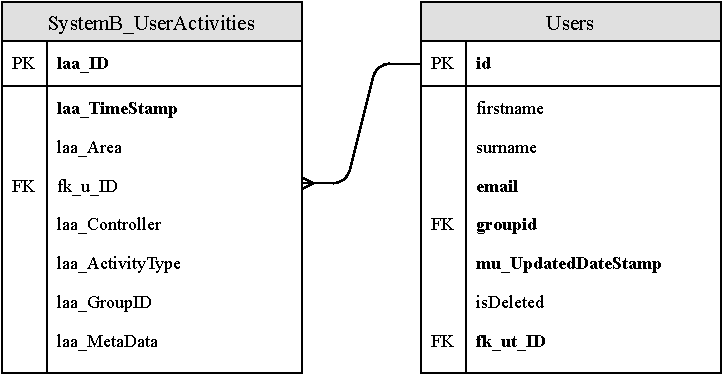
\includegraphics[width=0.99\textwidth]{Chapter2/SystemB_ERD_Basic/SystemB_ERD_Basic.pdf}
	\caption[ERD of user activities]
	{\textit{ERD of the user activities}}\label{fig:ch2:erdOfEventLogs}
\end{figure}

\clearpage

\section{System utilisation analysis}\label{ch2:system_utilisation_analysis}

\section{Integration}

\section{Conclusion}